\documentclass[10pt, a4paper]{article}

%Margins
%\usepackage[a4paper, total={6in, 9in}]{geometry}


\usepackage[utf8]{inputenc}
\usepackage[a4paper]{geometry}
\usepackage{enumitem}
\usepackage[table,xcdraw]{xcolor}
\usepackage{graphicx}
\usepackage{subcaption}
\usepackage{todonotes}
\usepackage{float}
\usepackage{multicol}
\usepackage{fancyhdr}
\usepackage{algorithm2e}
\usepackage{amsmath}
\usepackage{booktabs}
\usepackage{pgf, tikz}
\usepackage[simplified]{pgf-umlcd}
\usepackage{hyperref}
\usepackage{ amssymb }

\hypersetup{
    colorlinks=true,
    linkcolor=blue,
    filecolor=magenta,      
    urlcolor=cyan,
}
 
\urlstyle{same}

% Cool paragraphs without forcing them with //
\edef\restoreparindent{\parindent=\the\parindent\relax}
\usepackage[parfill]{parskip}
\restoreparindent

% Remove space on itemize items.
\setlist{nolistsep}


% Headings of each page
\pagestyle{fancy}
\lhead{Asaf Badouh}
\rhead{Laura Cebollero}
\cfoot{Page \thepage}
\renewcommand{\headrulewidth}{0.4pt}
\renewcommand{\footrulewidth}{0.4pt}


%%%%%%%%%%%%%%%%%%%%%
%%%% Doc info %%%%%%%
%%%%%%%%%%%%%%%%%%%%%
\title{ \Large  Information Retrieval \\ Lab 03 \\ \huge \textbf{Page-Rank implementation}}

\author{\textsc{Badouh, Asaf} \\ \textsc{Cebollero, Laura }}
\date{6th of November, 2018}

%%%%%%%%%%%%%%%%%%%%%

\begin{document}

% Remove page numbering on cover
\pagenumbering{gobble}

\maketitle
\begin{figure}[b!]
    \centering
    \includegraphics[width=\linewidth]{openflights-apdb-2048.png}
\end{figure}


\newpage

% Restore page numbering after cover!
\pagenumbering{Roman}

\section{Introduction}
In this lab we want to compute the page rank of airports using the network defined by routes from and to airports. For that, we used the supplied data downloaded from  \href{https://openflights.org/data.html}{\textit{Open flights}}\footnote{More details about the data structure can be found in the lab:  \href{http://www.cs.upc.edu/~ir-miri/labs/session3.zip}{Session03}}, which has been provided to us:
\begin{itemize}
    \itemsep-0.5em 
    \item {\fontfamily{qcr}\selectfont airport.txt} - contains a list of airports (\textbf{nodes}) from the world.
    \item {\fontfamily{qcr}\selectfont routes.txt} - contains a list of routes (\textbf{edges}) from the world.
\end{itemize}
As explained in the lab statement, we can represent this information as a graph, where airports are nodes and routes are edges. The \textbf{weights of the edges }will be the \textbf{number of flights between two airports}. Thus, \textbf{airports} with a \textbf{high PageRank} value are \textbf{\textit{important} airports}. 

This is crucial information for example when designing and reforming airports, as it means that many flights (either with passengers or goods) visit it when landing or taking off. In other words, they may be affected by such remodellings. 

Optimizing the operations of such important airports will lead to improvement of many supply chains and other visitors.

\section{Implementation Scheme}
Having described and seen the problem at hand, we will focus now on how the implementation of the airport has been done. We have chosen to stick to \textsc{Python} for this project.

Since some base code has been provided to us, we will focus mainly on two aspects:
\begin{itemize}
    \item The \textbf{data structures} we have settled on after implementation for both the nodes and edges.
    \item The \textbf{difficulties} we have faced, as well as the \textbf{decisions} taken to afront them.
\end{itemize}

\subsection{Data Structures}
As described on the introduction, there are only two main data structures:
\begin{itemize}
    \item The nodes, which act as Airports.
    \item The edges, which represents the \textit{directed} routes between two airports.
\end{itemize}

To create the nodes we have read them from the file {\fontfamily{qcr}\selectfont airport.txt}.

While analyzing it and creating our data structure, we have found a total of $7,663$ airport records. However, we have found some special cases:
\begin{enumerate}
    \item From the total, $1,923$ of them don't have IATA code, which is what we are using as an identifier for the airport.
    \item There is an airport that appears twice, so it is listed $2$ times on the file.
\end{enumerate}

To avoid having duplicates and working with airports with a missing identifier, we have discarded them. \textbf{This has left us  with a total $5,738$ \textit{valid} airports}. 

If we were to represent the problem in a two-dimensional array, that is, a matrix, it would consume a large size of bytes. Namely:  $$size = \thicksim 2^{25}\times sizeof(datatype)$$

Since the maximum weight found is $534$ (ORD - Chicago Ohare Intl, United States) our datatype must be at least 2-bytes, \textit{i.e. total of 64 Mega-Bytes}. 

This hypothetic \textbf{matrix would be very sparse}, so in order to save data space \footnote{In fact, 64MB is not that big nowadays, in efficiency terms it might even be better to save the data as matrix in order to save data manipulation and random accesses. Nevertheless, we have chosen to stick to the skeleton structures provided.}, we have decided to save the information in two dictionaries, one for each structure: airports and routes.

Below, in figure \ref{fig:uml}, you can see how the structures have ended up being defined. 
\begin{figure}[h]
    \centering
    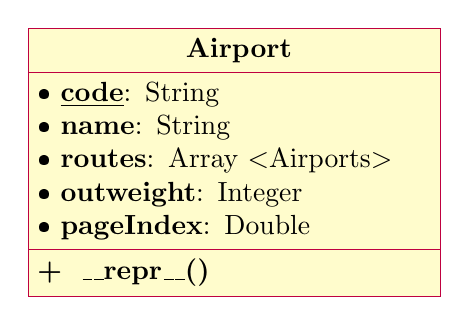
\begin{tikzpicture}
    \begin{class}[text width = 5cm]{ Airport }{0 ,0}
        \attribute {\textbullet \  \textbf{\underline{code}}: String}
        \attribute {\textbullet \ \textbf{name}: String}
        \attribute {\textbullet \ \textbf{routes}: Array \textless Airports\textgreater}
        \attribute {\textbullet \ \textbf{outweight}: Integer}
        \attribute {\textbullet \ \textbf{pageIndex}: Double}
        \operation {\textbf{+ \ \_\_repr\_\_()} }
    \end{class}
    \end{tikzpicture}
    \hspace{5pt}
    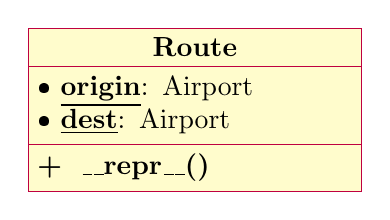
\begin{tikzpicture}
    \begin{class}[text width = 4cm]{Route}{0 ,0}
        \attribute {\textbullet \  \textbf{\underline{origin}}: Airport }
        \attribute {\textbullet \  \textbf{\underline{dest}}: Airport }
        \operation {\textbf{+ \ \_\_repr\_\_()} }
    \end{class}
    \end{tikzpicture}
\caption{Class diagrams}
\label{fig:uml}
\end{figure}


Each attribute of the \textbf{airport} consists of:
\begin{itemize}
    \item \textbf{code}: IATA airport code. Identifier of the airport.
    \item \textbf{name}: Airport name.
    \item \textbf{routes}: List of all airports that have a route that points to the current airport. In other words, list of airports that have as a destination this airport.
    \item \textbf{outweight}: Number of departure flights from this airport.
    \item \textbf{pageIndex}: Page-rank index.
\end{itemize}

As for the Route structure, its structure is way simpler:
\begin{itemize}
    \item \textbf{Origin}: The airport from where the flight takes off.
    \item \textbf{Dest}: The destination airport, where the flight will land on.
\end{itemize}


The \texttt{repr} function in both structures just defines how the airport and route should be defined.

\subsection{Difficulties and Choices}
\noindent\fbox{%
    \parbox{\textwidth}{%
        \textcolor{red}{Laura!! I tried here to answer this question from the lab:} Modify the pseudocode above to add the effect of these (virtual) edges efficiently: how many of them are there, and how much pagerank do they add in total to each vertex in particular?
    }%
}
Our main difficulty was dealing with the \textit{airports} without departures(formally, \textit{dangling nodes}). There are three accepted approaches for treating pages with no outgoing links\cite{pageRank}:
\begin{enumerate}
    \item Eliminate such pages from the graph (iteratively prune the graph until reaching a steady state).
    \item Consider such pages to link back to the pages that link to them.
    \item Consider such pages to link to all web pages (effectively making an exit out of them equivalent to a random jump).
\end{enumerate}
The first approach can lead to loss of information. consider the graph in figure[\ref{graph:s0}] that represent our network, we can see that we can lose information about airports. The second and third approaches are more robust and promise that we will not lose information, we decided to add link to all nodes \textcolor{red}{(TRUE??)}. However, we don't keep it on the data structure itself, we add it to the iterative computation of the page-rank, therefore we won't "pay" for $n^2$ new edges.
\usetikzlibrary{arrows, automata, positioning}
\begin{figure}[h!]
    \begin{minipage}{0.24\textwidth}
    \scalebox{0.7}{
    \begin{tikzpicture}[
            > = stealth, % arrow head style
            shorten > = 1pt, % don't touch arrow head to node
            auto,
            node distance = 2cm, % distance between nodes
            semithick % line style
        ]
    
        \tikzstyle{every state}=[
            draw = black,
            thick,
            fill = white,
            minimum size = 4mm
        ]
    
        \node[state] (TLV) {$TLV$};
        \node[state] (BCN) [right of=TLV] {$BCN$};
        \node[state] (KOA) [below  of=BCN] {$KOA$};
        \node[state] (SYD) [below of=TLV] {$SYD$};
        \path[->] (TLV) [] edge node { } (BCN);
        \path[->] (BCN) [] edge node { } (KOA);
        \path[->] (KOA) [] edge node { } (SYD);
    \node[above,font=\bfseries] at (current bounding box.north) {Initial state\\};
    \end{tikzpicture}}
    \end{minipage}
    \begin{minipage}{0.24\textwidth}
    \scalebox{0.7}{
    \begin{tikzpicture}[
            > = stealth, % arrow head style
            shorten > = 1pt, % don't touch arrow head to node
            auto,
            node distance = 2cm, % distance between nodes
            semithick % line style
        ]
    
        \tikzstyle{every state}=[
            draw = black,
            thick,
            fill = white,
            minimum size = 4mm
        ]
    
        \node[state] (TLV) {$TLV$};
        \node[state] (BCN) [right of=TLV] {$BCN$};
        \node[state] (KOA) [below  of=BCN] {$KOA$};
        
        \path[->] (TLV) [] edge node { } (BCN);
        \path[->] (BCN) [] edge node { } (KOA);
        \node[above,font=\bfseries] at (current bounding box.north) {1st iteration - remove SYD};
    \end{tikzpicture}
    }
    \vfill
    \end{minipage}
    \begin{minipage}{0.24\textwidth}
    \scalebox{0.7}{
    \begin{tikzpicture}[
            > = stealth, % arrow head style
            shorten > = 1pt, % don't touch arrow head to node
            auto,
            node distance = 2cm, % distance between nodes
            semithick % line style
        ]
    
        \tikzstyle{every state}=[
            draw = black,
            thick,
            fill = white,
            minimum size = 4mm
        ]
    
        \node[state] (TLV) {$TLV$};
        \node[state] (BCN) [right of=TLV] {$BCN$};
        
        \path[->] (TLV) [] edge node { } (BCN);
                \node[above,font=\bfseries] at (current bounding box.north) {2nd iteration - remove KOA};
    \end{tikzpicture}}
    \end{minipage}
    \begin{minipage}{0.24\textwidth}
    \scalebox{0.7}{
    \begin{tikzpicture}[
            > = stealth, % arrow head style
            shorten > = 1pt, % don't touch arrow head to node
            auto,
            node distance = 2cm, % distance between nodes
            semithick % line style
        ]
    
        \tikzstyle{every state}=[
            draw = black,
            thick,
            fill = white,
            minimum size = 4mm
        ]
        \node[state] (TLV) {$TLV$};
        \node[above,font=\bfseries] at (current bounding box.north) {3rd iteration - remove BCN};
    \end{tikzpicture}
    }
    \end{minipage}
    \caption{1st approach}
    \label{graph:s0}
\end{figure}




\section{Experiments and Observations}
different dumping factors
about the converges parameter
other?


\newpage
\nocite{*}
\bibliographystyle{unsrt}
\bibliography{references}
\end{document}
